\documentclass[12pt,a4paper]{article}
\usepackage[width=.75\textwidth]{caption}
\usepackage{amsfonts}
\usepackage{amsmath}
\usepackage{amssymb}
\usepackage{authblk}
\usepackage{braket}
\usepackage{epigraph}
\usepackage{fancyhdr}
\usepackage{graphicx}
%\usepackage{mathrsfs}
\usepackage[mathscr]{euscript}
\usepackage[top=2cm, bottom=2cm, left=2cm, right=2cm]{geometry}

\setlength{\epigraphwidth}{0.8\textwidth}

% \pagestyle{fancy}
\begin{document}

%title and author details
\title{Spacetime from Matter Wave Emanations}
\author[1]{Kevin Player\footnote{kjplaye@gmail.com}}

\maketitle


\epigraph{After long reflection in solitude and meditation, I suddenly had the idea, during the year 1923, that the discovery made by Einstein in 1905 should be generalised by extending it to all material particles and notably to electrons.}{Louis de Broglie}


\abstract{Einstein taught us that matter is not a passive actor in mechanics, but that it actually shapes and defines the very spacetime it occupies.  In a similar vein, we turn our attention to De Broglie's matter waves and show how they can actively shape and define space and time as intrinsic properties of massive particles. For two particles, we equate the frequencies of a quantum superposition with the De Broglie frequencies of interacting matter in a gravitational setting. Through this we produce a ratio of energies, quantum scale energy and gravitational self-energy, that connect to quantum gravity and black hole information theory.  This is particularly clear when this ratio equals one at an event horizon.}

\section{Introduction}
How can we quantize gravity without quantizing spacetime (or at least curvature)? And how can we do QFT computations in a probabilistic discrete spacetime?  It may be that these issues must be dealt with when trying to understand quantum gravity.  One may take the view that spacetime is made up of a mesh of Planck scale lengths and times, but this is not immediately Lorentz invariant and seems to side step the issues.  We instead take the viewpoint that space and time are actually properties of matter; that spacetime only makes sense up to the resolution of the matter emanating it.  Using matter waves to do this grants us automatic Lorentz invariance.  The approach allows us to define a system where emergent proper time and space can be compared to gravity at classical scales.

In this short note we explore how matter waves \cite{debroglie} and the Compton ``clock'' \cite{clock} can be used to connect quantum mechanics and gravity at a basic level.  We express time and space as properties of matter in both settings by counting ``ticks''.  The number of ticks is an internal property of matter, akin to an emergent proper time from general relativity.

In the first section we formalize ``counting ticks'' for a massive particle to understand time as an emergent propery.  In the next section we study phase differences of a superposition of clocks to understand space as an emergent propery.  Then we develop some equations that come out of comparing matter waves in the quantum realm to the gravitational.

\section{Counting Ticks for Emergent Time}

Recall that a massive particle with mass $m$, such as an electron, has a DeBroglie frequency:

\begin{equation}
\label{debroglie_eq}
\omega = \frac{c^2}{\hslash} m
\end{equation}
We will discuss the number of ``ticks'', at frequency $\omega$, that the particle has undergone from time $t_1$ to $t_2$ by unwrapping the phase of the particle and identifying the lifted zero crossings.

\[
    T_{t_1,t_2}(e^{i \omega t} \rightarrow t) = \{ t \in [t_1,t_2]: t \in \frac{2 \pi}{\omega} \mathbb{Z} \}
\]
In this context, $\omega$ functions like a sampling rate or Nyquist rate for the matter in ticks per second.  This concept parallels Bremermann's limit where the constant $\frac{c^2}{\hslash}$ that we see in equation (\ref{debroglie_eq}) represents ticks per second per kg.  The Bremermann context was also that of a clock, placing limits on computation via material ``CPU clocks''.


We treat the number of ticks, $|T|$ , as a quantum observable.  In fact we may not know the bounds $t_1,t_2$ but can still sometimes talk about the distribution of number of ticks between two events such as particle emissson and detection.  The number of ticks is a wave function $\varphi$ in the Hilbert space $H(T)$,
\[
   H(T) = \mathrm{Span}(\ket{0}, \ket{1}, \cdots)
\]
It will act as an emergent representation of time for the particle. Since the number of ticks is relative to the particle itself, and not to an external observer, it resembles most closely the concept of proper time.  In particular, the number of tick is Lorentz invariant.

\section{Double Slit for Emergent Space}


\begin{figure}[h!]
\centering
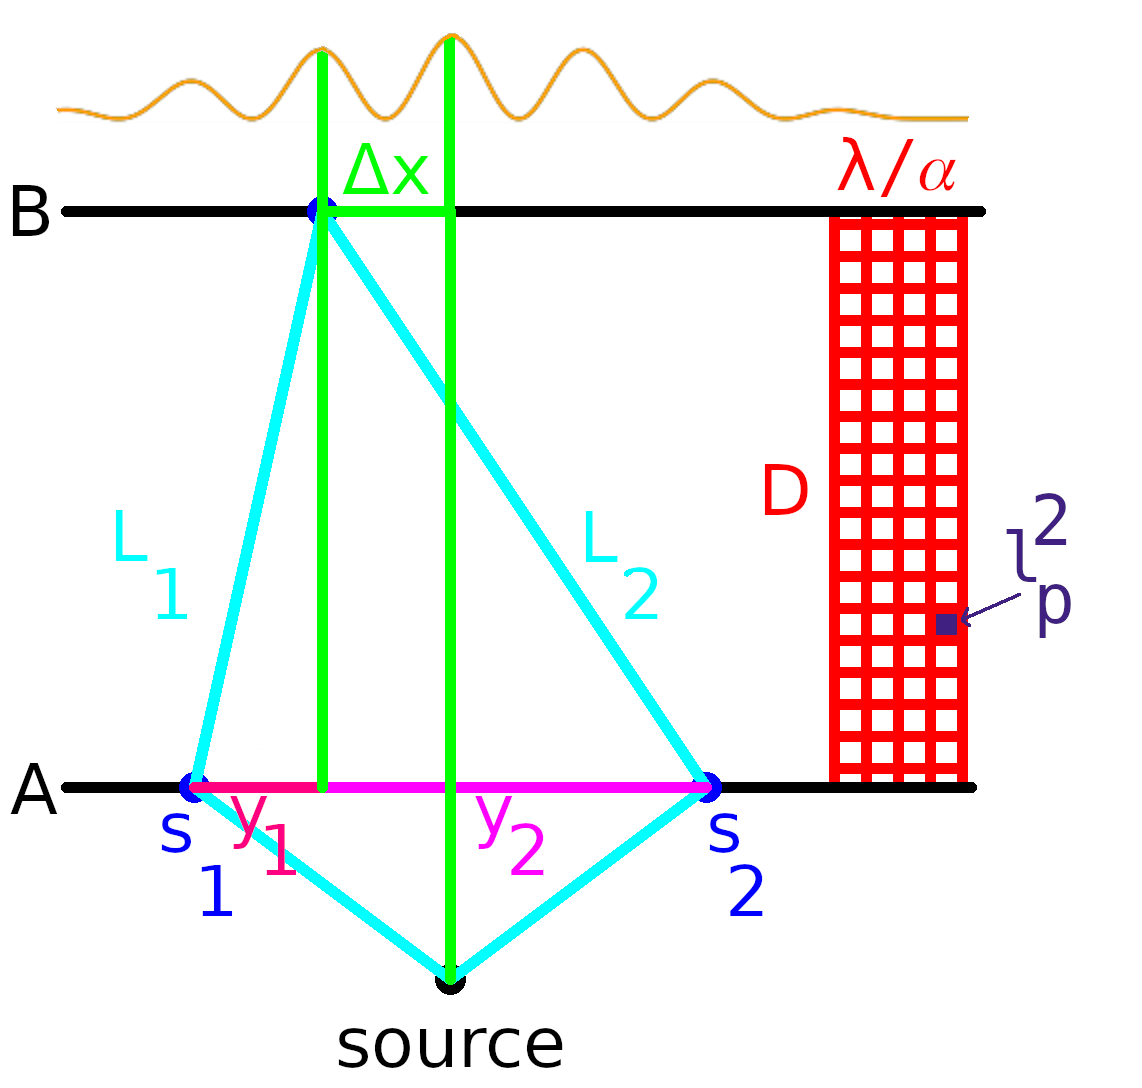
\includegraphics[scale=0.5]{double_slit.png}
\caption{Typical double slit setup.  $D$ is the distance between screens $A$ and $B$. $\Delta s = s_2 - s_1$ is the distance between slits.  $\Delta x$ is the distance between constructive fringes. $\Delta L = \lambda$ is the difference of path lengths.  $\frac{\lambda D}{l_p^2} = \alpha$ is a ``count'' of Planck length squares.}
\label{screen}
\end{figure}


Consider the situation in Figure \ref{screen}.  The particle of mass $m$ is in quantum superposition, going through two slits, $s_1$ and $s_2$, on a one dimensional screen $A$. Let B be another screen behind $A$ with distance $D$ between them. Then for any time $t$ and position $x$, beyond $s_1$ and $s_2$, we have the number of ticks; $n_1$ with repect to $s_1$, and $n_2$ with repect to $s_2$. So $(n_1,n_2)$ is a function of $(t,x)$. Note that the interference patterns that appear on a screen $B$ are given by fringes of constructive interference each of which can be labeled by a unique $k = n_2 - n_1$.

Similar to how we model time using ticks, we can use the phase offset of the ticks, $k$, to model space. We describe how space emerges as a property of the massive particle by considering the Hilbert space for both paths jointly $H(T_1,T_2)$
\[
\begin{split}
  H(T_1,T_2) &= H(T_1) \otimes H(T_2) \\
  & = \mathrm{Span}(\{\ket{i} \otimes \ket{j}: i,j \in \mathbb{Z}_{\ge 0}\}) \\
  & = \sum_{k \in \mathbb{Z}} \mathrm{Span}(\{\ket{i} \otimes \ket{j} : i,j \in \mathbb{Z}_{\ge 0}, i-j = k\}) \\
\end{split}
\]
Then we consider the projection-valued measure $\{\Pi_k\}$ that picks out the space-like fringes, where $k$ labels the summands spaces above.

Let $L_1$ and $L_2$ be the lengths of the path from the source to the screen for the particle going through $s_1$ and $s_2$ respectively. Let the particle have a wavelength of $\lambda = \Delta L$ and we consider the first noncentral fringe, $k=1$, at distance $\Delta x$ away from the center.  We have $L_i = \sqrt{y_i^2 + D^2}$ and approximating the square root we have $\lambda \approx \frac{\Delta s \Delta x}{D}$.

\subsection{Double Slit Tick Equations}
Back to the one dimensional screen case.  Consider the local behaviour of the interference pattern near the middle of $B$ (the central fringe $k=0$). The fringe pattern is locally made up of a combination of a part in space (fringes) and a part in time (particle evolution). Let $n_{1,2} = (n_1, n_2)$ label the antinodes of this pattern in space-time. The antinodes each pick out individual $n_{1,2}$ values, associated with the zero phase. We can write out a 2d joint frequency $\nu = \omega^2$ (in Hz * Hz) of this pattern using $\Delta x$ and $\Delta t$.  Using the mass energy of the particle $E_\hslash = \hslash \omega = \frac{\hslash}{\Delta t}$, we have
\begin{equation}
\label{nu_h}
  \nu = \frac{c}{\Delta x \Delta t} = \frac{c}{\hslash \lambda D} E_\hslash \Delta{s}
\end{equation}
and
\begin{equation}
\label{def_h}
E_\hslash = m c^2
\end{equation}


Following suit with Penrose\cite{penrose} we let $E_G$ approximate the gravitational (self) energy of the particle 
\begin{equation}
\label{def_G}
E_G = \frac{G m^2}{\Delta s}
\end{equation}
Using the gravitational potential and setting $\omega^2$  equal to $m^2$ times the squared Bremermann constant $c^4/\hslash^2$ we have
\begin{equation}
\label{nu_G}
\nu = \omega^2 = \frac{c^4}{G \hslash^2} E_G \Delta s
\end{equation}


We have written $\nu$ in two ways, equations (\ref{nu_h}) and (\ref{nu_G}). Setting these two representations of $\nu$ equal to each other we get
\begin{equation}
\label{count}
\lambda D = \frac{E_\hslash}{E_G} l_p^2 = \alpha l_p^2
\end{equation}
where $l_p = \sqrt{\frac{\hbar G}{c^3}}$ is the Planck length and we define $\alpha = \frac{E_\hslash}{E_G}$. Equation (\ref{count}) suggestively counts Planck areas in $\lambda D$ in terms of the unitless $\alpha$:
\begin{equation}
\label{count2}
   \alpha = \frac{\lambda D}{l_p^2}
\end{equation}


\subsection{Escape Velocity, $\alpha$, and Black Holes}
We have another way of understanding $\alpha$.  By using equations (\ref{def_h}) and (\ref{def_G}) we have
\begin{equation}
\label{escape}
  \frac{1}{\alpha} = \frac{E_G}{E_\hslash} = \frac{Gm}{c^2\Delta s} = \left(\frac{v_e}{c}\right)^2
\end{equation}
where $v_e$ is an escape velocity for diameter $\Delta s$.  With this understanding we must have
\begin{equation}
\label{ine}
   E_\hslash \ge E_G
\end{equation}
and
\begin{equation}
\label{alphaone}
  \alpha \ge 1 
\end{equation}
The following are equivalent
\begin{enumerate}
\item $E_\hslash = E_G$
\item $v_e = c$
\item $\alpha = 1$
\item The particle is a black hole.
\end{enumerate}
In the black hole case the suggestive count of $\alpha$ in equation (\ref{count2}) is related to the count of Planck areas on the event horizon.  To see this let the surface area of the black hole be $A = 4 \gamma \lambda D$.  In black hole thermodynamics \cite{bekenstein}, we have an entropy $S_\text{BH} = \frac{A}{4 l_p^2}$ and we can compute

\[
  S_\text{BH} = \frac{A}{4 l_p^2} = \frac{\gamma \lambda D}{l_p^2} = \gamma \alpha = \gamma \text{ (nats) }
\]

\subsection{Information and Acceleration}

The treatment in this note extends to the less exotic $v_e < c$ case.  For the Schwarzschild metric we have a unitless time dialation factor $\tau = \sqrt{1 - \left(\frac{v_e}{c}\right)^2}$.  Using equation (\ref{escape}) we can relate this to the unitless $\alpha$ by writing
\[
\tau = \sqrt{1 - \frac{1}{\alpha}}
\]


\subsection{Appendix: Triple Holes Set up}

The situation in three dimensions is similar which we breifly cover.  Suppose we have three holes in a two dimensional screen with another screen behind it.  We then have three tick counters $n_1$, $n_2$ and $n_3$ and there is a two dimensional space indexing the 2d fringe pattern by the two dimensional space spanned by $n_1 - n_2$ and $n_1 - n_3$.  We could add more holes as well.

\begin{figure}[h!]
\centering
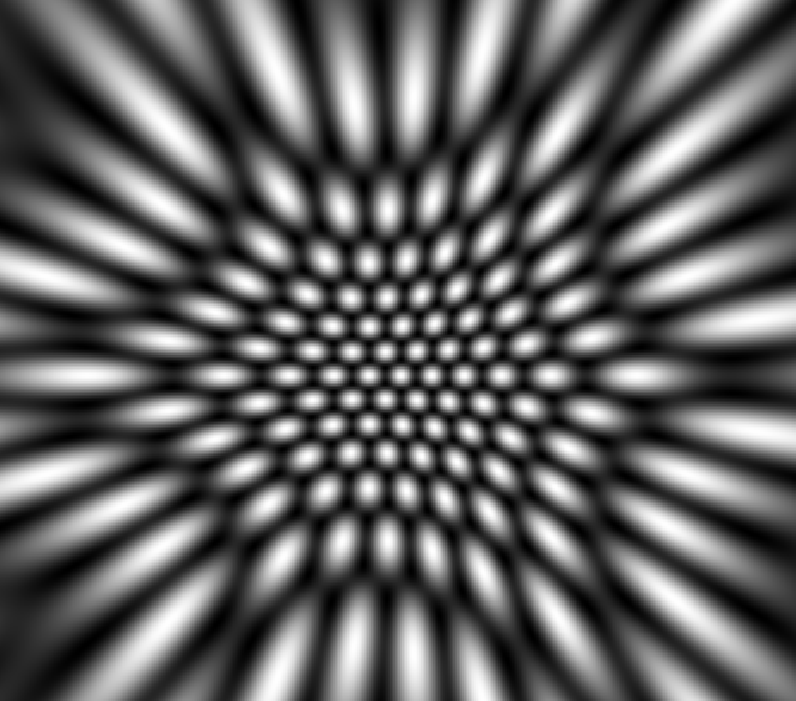
\includegraphics[scale=0.5]{triple_hole.png}
\caption{Fringe pattern on 2d screen behind a triple hole.}
\label{screen}
\end{figure}


\section{TODO}
\begin{enumerate}
\item $\hslash$ vs $h$
\item Entropy for general case?
\item What do the wavefunctions mean?
\item 3d case?
\item Dirac equation
\end{enumerate}

\begin{thebibliography}{10}

\bibitem{bekenstein} Bekenstein, A. (1972). "Black holes and the second law". Lettere al Nuovo Cimento. 4 (15): 99–104. doi:10.1007/BF02757029. S2CID 120254309.
\bibitem{debroglie} de Broglie, Louis Victor. "On the Theory of Quanta" (PDF). Foundation of Louis de Broglie (English translation by A.F. Kracklauer, 2004. ed.). Retrieved 25 February 2023.
\bibitem{clock}  Lan, S-Y et al.; "A Clock Directly Linking Time to a Particle's Mass", Science 1 February 2013: Vol. 339 no. 6119 pp. 554–557 doi:10.1126/science.1230767
\bibitem{penrose} Penrose, R. On the Gravitization of Quantum Mechanics 1: Quantum State Reduction. Found Phys 44, 557–575 (2014). https://doi.org/10.1007/s10701-013-9770-0

\end{thebibliography}

\end{document}

